\section{Results}

The central result is that the frozen zero-shot teacher remains the strongest point in the study, while naive shallow compression collapses retrieval quality unless the query tower is handled carefully. Table~\ref{tab:main-results} summarizes the quality tradeoffs, Table~\ref{tab:latency-results} summarizes online behavior, and Table~\ref{tab:ann-results} reports the exact-versus-ANN comparison.

\begin{figure}[t]
\centering
\resizebox{\columnwidth}{!}{% Standalone TikZ fragment for \input into the paper body.
% Assumes the document preamble already loads tikz and amsmath.
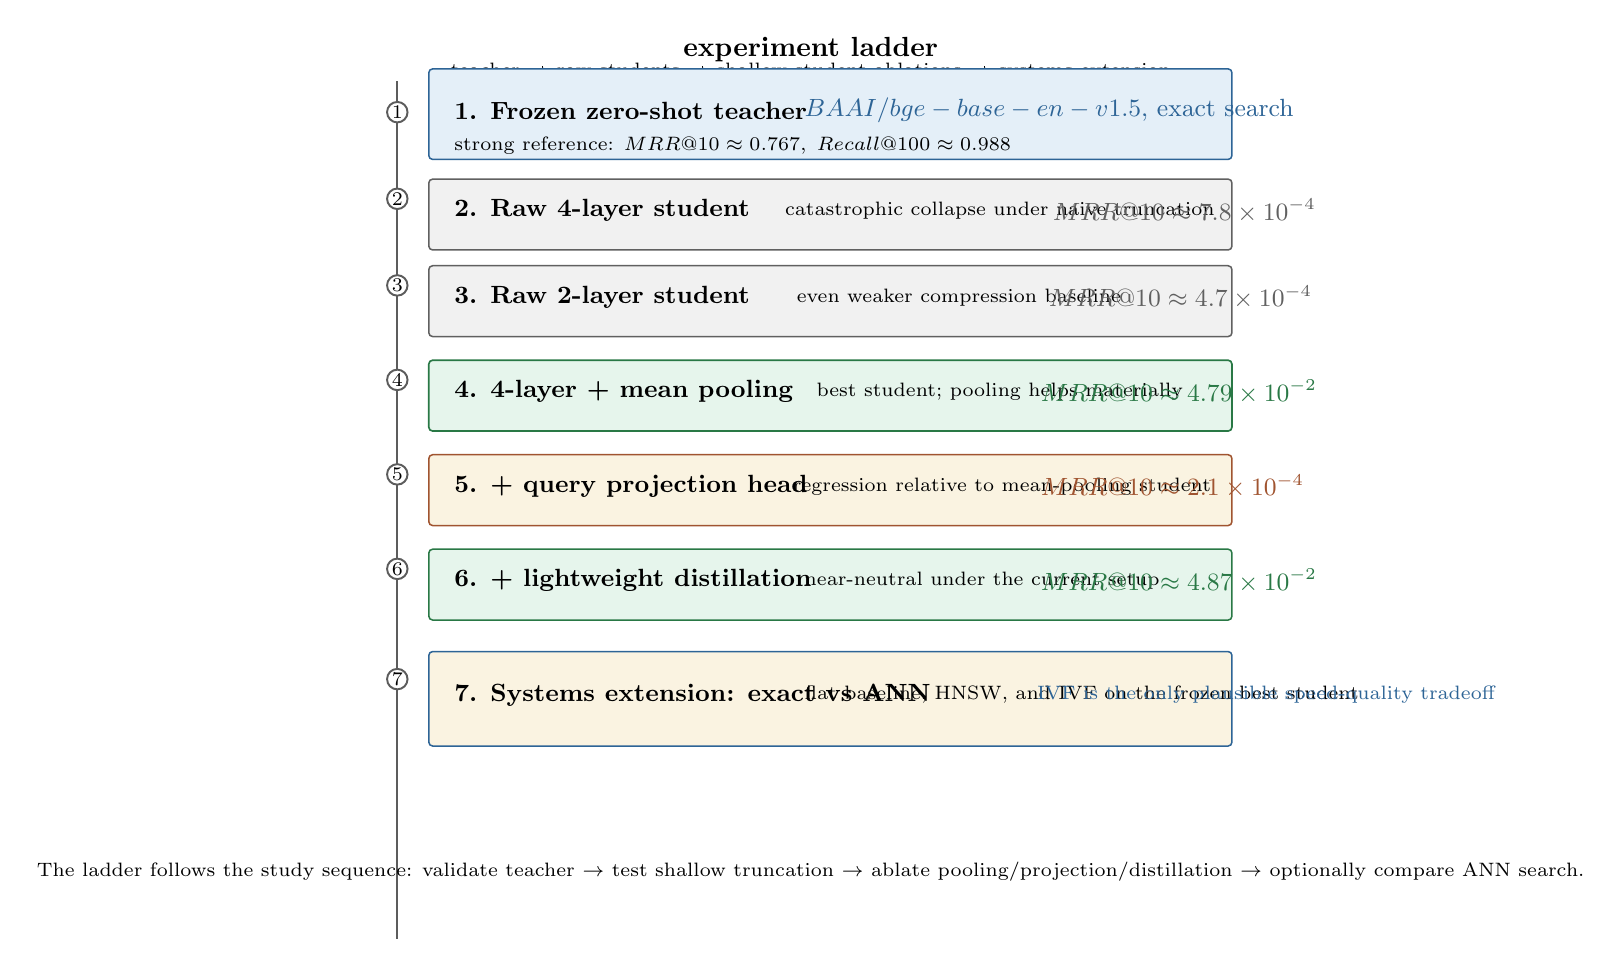
\begin{tikzpicture}[x=1cm,y=1cm, font=\small]
  \definecolor{stageblue}{RGB}{228,239,248}
  \definecolor{stagegray}{RGB}{241,241,241}
  \definecolor{stagegreen}{RGB}{230,245,236}
  \definecolor{stagered}{RGB}{250,233,233}
  \definecolor{stageamber}{RGB}{250,243,225}
  \definecolor{stepline}{RGB}{92,92,92}
  \definecolor{teacherline}{RGB}{45,100,150}
  \definecolor{studentline}{RGB}{96,96,96}
  \definecolor{bestline}{RGB}{41,120,69}
  \definecolor{warnline}{RGB}{160,84,48}

  % Vertical spine for the "ladder" metaphor.
  \draw[line width=0.7pt, draw=stepline] (0.95,0.7) -- (0.95,11.6);

  % Step markers.
  \foreach \yy/\lab in {11.2/1,10.1/2,9.0/3,7.8/4,6.6/5,5.4/6,4.0/7} {
    \fill[white] (0.95,\yy) circle (0.13);
    \draw[line width=0.7pt, draw=stepline] (0.95,\yy) circle (0.13);
    \node[font=\scriptsize] at (0.95,\yy) {\lab};
  }

  % Top annotation.
  \node[align=left, font=\bfseries] at (6.2,12.0) {experiment ladder};
  \node[align=left, font=\scriptsize] at (6.2,11.72) {teacher \textrightarrow\ raw students \textrightarrow\ shallow-student ablations \textrightarrow\ systems extension};

  % Step 1: teacher reference.
  \draw[rounded corners=1.4pt, line width=0.55pt, draw=teacherline, fill=stageblue] (1.35,10.6) rectangle (11.55,11.75);
  \node[anchor=west, align=left] at (1.55,11.22) {\textbf{1. Frozen zero-shot teacher}};
  \node[anchor=west, align=left, text=teacherline] at (6.0,11.22) {$\text{BAAI/bge-base-en-v1.5}$, exact search};
  \node[anchor=west, align=left] at (1.55,10.78) {\scriptsize strong reference: $MRR@10 \approx 0.767,\; Recall@100 \approx 0.988$};

  % Step 2: raw four-layer student.
  \draw[rounded corners=1.4pt, line width=0.55pt, draw=studentline, fill=stagegray] (1.35,9.45) rectangle (11.55,10.35);
  \node[anchor=west, align=left] at (1.55,9.95) {\textbf{2. Raw 4-layer student}};
  \node[anchor=west, align=left] at (5.75,9.95) {\scriptsize catastrophic collapse under naive truncation};
  \node[anchor=west, align=left, text=studentline] at (9.15,9.95) {$MRR@10 \approx 7.8\times10^{-4}$};

  % Step 3: raw two-layer student.
  \draw[rounded corners=1.4pt, line width=0.55pt, draw=studentline, fill=stagegray] (1.35,8.35) rectangle (11.55,9.25);
  \node[anchor=west, align=left] at (1.55,8.85) {\textbf{3. Raw 2-layer student}};
  \node[anchor=west, align=left] at (5.9,8.85) {\scriptsize even weaker compression baseline};
  \node[anchor=west, align=left, text=studentline] at (9.1,8.85) {$MRR@10 \approx 4.7\times10^{-4}$};

  % Step 4: best positive pooling ablation.
  \draw[rounded corners=1.4pt, line width=0.6pt, draw=bestline, fill=stagegreen] (1.35,7.15) rectangle (11.55,8.05);
  \node[anchor=west, align=left] at (1.55,7.65) {\textbf{4. 4-layer + mean pooling}};
  \node[anchor=west, align=left] at (6.15,7.65) {\scriptsize best student; pooling helps materially};
  \node[anchor=west, align=left, text=bestline] at (9.0,7.65) {$MRR@10 \approx 4.79\times10^{-2}$};

  % Step 5: projection head ablation.
  \draw[rounded corners=1.4pt, line width=0.55pt, draw=warnline, fill=stageamber] (1.35,5.95) rectangle (11.55,6.85);
  \node[anchor=west, align=left] at (1.55,6.45) {\textbf{5. + query projection head}};
  \node[anchor=west, align=left] at (5.85,6.45) {\scriptsize regression relative to mean-pooling student};
  \node[anchor=west, align=left, text=warnline] at (9.0,6.45) {$MRR@10 \approx 2.1\times10^{-4}$};

  % Step 6: lightweight distillation.
  \draw[rounded corners=1.4pt, line width=0.55pt, draw=bestline, fill=stagegreen] (1.35,4.75) rectangle (11.55,5.65);
  \node[anchor=west, align=left] at (1.55,5.25) {\textbf{6. + lightweight distillation}};
  \node[anchor=west, align=left] at (6.0,5.25) {\scriptsize near-neutral under the current setup};
  \node[anchor=west, align=left, text=bestline] at (9.0,5.25) {$MRR@10 \approx 4.87\times10^{-2}$};

  % Step 7: ANN extension.
  \draw[rounded corners=1.4pt, line width=0.55pt, draw=teacherline, fill=stageamber] (1.35,3.15) rectangle (11.55,4.35);
  \node[anchor=west, align=left] at (1.55,3.8) {\textbf{7. Systems extension: exact vs ANN}};
  \node[anchor=west, align=left] at (6.0,3.8) {\scriptsize flat baseline, HNSW, and IVF on the frozen best student};
  \node[anchor=west, align=left, text=teacherline] at (8.95,3.8) {\scriptsize IVF is the only plausible speed-quality tradeoff};

  % Footer annotation.
  \node[align=left, font=\scriptsize] at (6.2,1.55) {The ladder follows the study sequence: validate teacher $\rightarrow$ test shallow truncation $\rightarrow$ ablate pooling/projection/distillation $\rightarrow$ optionally compare ANN search.};
\end{tikzpicture}
}
\caption{Experiment ladder for the study: frozen teacher, raw shallow students, low-cost ablations, and then the optional ANN systems extension.}
\label{fig:ladder}
\end{figure}

\subsection{Retrieval quality}

The frozen teacher reference, \texttt{BAAI/bge-base-en-v1.5} with \textsc{cls} pooling, achieves $\mathrm{MRR}@10 = 0.766997$ and $\mathrm{Recall}@100 = 0.988237$ on the prepared MS MARCO slice. The conservative fine-tuned teacher remains slightly worse at $0.740860 / 0.983169$, so the paper uses the zero-shot model as the teacher reference rather than the fine-tuned ablation.

The shallow student results show a large quality cliff. The raw 4-layer student reaches only $0.000776 / 0.016888$, and the 2-layer student is even weaker at $0.000465 / 0.010698$. This is the clearest evidence that naive query truncation is not a viable compression strategy under the current setup.

Among the student ablations, query-side mean pooling is the first clearly positive intervention. The 4-layer student with mean pooling improves to $0.047922 / 0.249231$, which is still far below the teacher but is orders of magnitude better than the raw shallow student. The query projection head is a regression: it drops to $0.000208 / 0.004516$. Lightweight distillation is near-neutral relative to the pooling-only student, nudging $\mathrm{MRR}@10$ to $0.048725$ while slightly lowering $\mathrm{Recall}@100$ to $0.246582$.

\subsection{Latency and systems behavior}

The latency measurements in Table~\ref{tab:latency-results} show that the student-side query encoder can be made materially cheaper, but exact end-to-end retrieval is still dominated by corpus search. The best 4-layer mean-pooling student reduces query p50 latency to $1.819$\,ms from $3.089$\,ms for the frozen teacher, yet end-to-end p50 latency remains similar at $25.243$\,ms versus $23.567$\,ms. The 2-layer student is faster than the teacher at query time, but its retrieval quality is too poor to justify the stronger compression. The projection-head and distillation variants do not meaningfully change the systems picture.

\subsection{ANN tradeoff}

Table~\ref{tab:ann-results} compares exact FAISS search against two approximate indices on the frozen best student. \texttt{HNSW} yields the fastest mean search time at $0.038$\,ms, but its retrieval quality drops sharply to $0.032009 / 0.147751$, which is too large a loss for the present study. \texttt{IVF} is the only ANN variant with a defensible tradeoff: it preserves much more of the exact-search quality at $0.044107 / 0.223453$ while reducing mean search time to $1.151$\,ms from $3.579$\,ms for exact search. For this benchmark, \texttt{IVF} is the only approximate index worth mentioning as a plausible systems compromise.

\begin{figure}[t]
\centering
\resizebox{\columnwidth}{!}{% Standalone PGFPlots fragment for \input into the paper body.
% Values are copied directly from the final ANN comparison for compile stability.
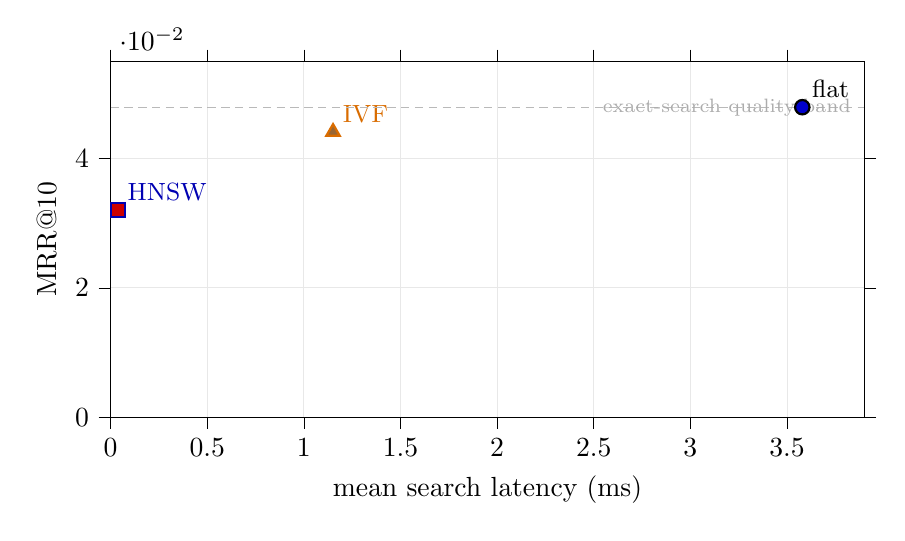
\begin{tikzpicture}
  \begin{axis}[
    width=0.92\linewidth,
    height=6.1cm,
    xlabel={mean search latency (ms)},
    ylabel={MRR@10},
    xmin=0,
    xmax=3.9,
    ymin=0.0,
    ymax=0.055,
    grid=both,
    major grid style={draw=gray!18},
    minor grid style={draw=gray!8},
    tick align=outside,
    tick style={black},
    legend style={draw=none, fill=none, at={(0.98,0.05)}, anchor=south east, font=\small},
    every axis plot/.style={line width=0.8pt},
    clip=false,
  ]
    % Exact search baseline.
    \addplot+[only marks, mark=*, mark size=2.6pt, color=black] coordinates {(3.5788,0.0479215)};
    \node[anchor=south west, font=\small] at (axis cs:3.5788,0.0479215) {flat};

    % HNSW and IVF.
    \addplot+[only marks, mark=square*, mark size=2.6pt, color=blue!70!black] coordinates {(0.0379,0.0320091)};
    \node[anchor=south west, font=\small, text=blue!70!black] at (axis cs:0.0379,0.0320091) {HNSW};

    \addplot+[only marks, mark=triangle*, mark size=2.8pt, color=orange!85!black] coordinates {(1.1511,0.0441068)};
    \node[anchor=south west, font=\small, text=orange!85!black] at (axis cs:1.1511,0.0441068) {IVF};

    % Readable contextual guides.
    \draw[densely dashed, gray!55] (axis cs:0,0.0479215) -- (axis cs:3.9,0.0479215);
    \node[anchor=east, font=\scriptsize, gray!65] at (axis cs:3.88,0.0479215) {exact-search quality band};
  \end{axis}
\end{tikzpicture}
}
\caption{ANN search-latency versus quality on the frozen best student. HNSW is fastest but too lossy; IVF retains much more of the exact-search quality while still reducing mean search latency.}
\label{fig:ann-tradeoff}
\end{figure}

\subsection{Transfer check}

As a small robustness check, the frozen best student transfers to SciFact with $\mathrm{MRR}@10 = 0.040016$ and $\mathrm{Recall}@100 = 0.326111$ on the BEIR evaluation run. This is far below the MS MARCO teacher reference, but it confirms that the student remains usable outside the in-domain benchmark.

\begin{table}[H]
\centering
\footnotesize
\renewcommand{\arraystretch}{1.05}
\caption{Retrieval quality on the prepared MS MARCO slice. The zero-shot teacher is the frozen reference model. The 4-layer mean-pooling student is the strongest student ablation, but it still trails the teacher by a wide margin.}
\label{tab:main-results}
\setlength{\tabcolsep}{4pt}
\begin{tabular}{@{}lrr@{}}
\toprule
Model & MRR@10 & Recall@100 \\
\midrule
Teacher Zero-Shot & 0.766997 & 0.988237 \\
Teacher Fine-Tune & 0.740860 & 0.983169 \\
Student Q4 CLS & 0.000776 & 0.016888 \\
Student Q2 CLS & 0.000465 & 0.010698 \\
Student Q4 Mean & 0.047922 & 0.249231 \\
Student Q4 Mean + Proj & 0.000208 & 0.004516 \\
Student Q4 Mean + Distill & 0.048725 & 0.246582 \\
\bottomrule
\end{tabular}
\end{table}

\begin{table}[H]
\centering
\footnotesize
\renewcommand{\arraystretch}{1.05}
\caption{Online behavior on the prepared benchmark. Query latency changes substantially across query encoders, but end-to-end latency remains dominated by exact corpus search. Peak memory is the measured query-side peak allocation during the latency evaluation, reported in MiB for readability.}
\label{tab:latency-results}
\setlength{\tabcolsep}{3.2pt}
\begin{tabular}{@{}lrrrr@{}}
\toprule
Model & q p50 & q p95 & e2e p50 & e2e p95 \\
\midrule
Teacher Zero-Shot & 3.089 & 3.199 & 23.567 & 23.821 \\
Teacher Fine-Tune & 3.075 & 3.213 & 23.837 & 24.243 \\
Student Q4 CLS & 7.171 & 8.206 & 31.239 & 32.680 \\
Student Q2 CLS & 4.107 & 4.478 & 24.800 & 25.405 \\
Student Q4 Mean & 1.819 & 1.991 & 25.243 & 26.183 \\
Student Q4 Mean + Proj & 1.848 & 1.957 & 24.822 & 25.105 \\
Student Q4 Mean + Distill & 1.824 & 1.999 & 23.172 & 23.902 \\
\bottomrule
\end{tabular}
\end{table}

\begin{table}[t]
\centering
\small
\caption{Exact FAISS versus approximate indices on the frozen best student. All rows use the same 55{,}578-query benchmark slice. \texttt{IVF} is the only approximate index that preserves most of the exact-search quality while still reducing mean search latency.}
\label{tab:ann-results}
\resizebox{\columnwidth}{!}{%
\begin{tabular}{llrrrrrl}
\toprule
Index & MRR@10 & Recall@100 & Build (s) & Search (s) & Mean search (ms) & Queries & Notes \\
\midrule
Flat & 0.047922 & 0.249231 & 0.450 & 198.904 & 3.579 & 55{,}578 & Exact FAISS baseline \\
HNSW & 0.032009 & 0.147751 & 32.043 & 2.108 & 0.038 & 55{,}578 & Fastest search, but large quality drop \\
IVF & 0.044107 & 0.223453 & 3.285 & 63.974 & 1.151 & 55{,}578 & Moderate speedup with smaller quality loss \\
\bottomrule
\end{tabular}
\par}
\end{table}

